\documentclass[12pt]{article}
\usepackage{amsmath}
\usepackage{graphicx}
\title{Interference Temperature \\ (Supervised Research Exposition)}
\author{Swrangsar Basumatary (Roll 09d07040) \\ \textbf{Guide:} \emph{Prof. S N Merchant}}
\date{April 2013}
\begin{document}


\maketitle

\begin{abstract}

The concept of interference temperature was introduced by the FCC as a new metric for quantifying and managing interference. Using this model, cognitive radios (CRs) operating in licensed frequency bands would be able to measure their current interference environment and adjust their transmission characteristics so as not to raise the interference temperature over a regulatory limit.

As of now it is hard to predict whether interference temperature is going to be practical because no one has been able to come up with a solution that is agreed upon by everyone. The research on interference temperature was abandoned by the Federal Communications Commission (FCC) in 2007 but there is some hope of a comeback.

This document highlights what I have learned about interference temperature as part of my supervised research exposition.

\end{abstract}

\section{Introduction}

The purpose of this metric (interference temperature) is to remove the subjective context that has been the basis of interference analysis up to now\cite{kolodzy2006}. The development of an interference metric is critical to making efficient use of the spectrum.

The current regulatory definition of interference is not precise. The process used by the regulatory bodies to estimate interference is slow. It is specific to particular deployment geometries and thereby cannot be automated. They usually do a  detailed analysis of the surroundings.

With the progress in technology, new devices have shown up that are capable of waveform modification and changing frequency of operation very quickly. These new devices have the potential to make more efficient use of the spectrum. But without a clear definition of interference, we will lose the ability to exploit these new technologies to harness the spectral resources. Performing detailed analysis for every combination of waveforms and receivers is not feasible.

Relying on worst case analysis leaves much of the spectrum unused. There is a need for some real-time interference metric so that we can make efficient use of the spectral resources that are available.

\section{Driving forces for interference metric}

Spectrum management revolves around interference management\cite{kolodzy2006}. The design and operation of all RF equipments is based on the idea of reducing electromagnetic interference. Interference limits the usable range of wireless signals.

\subsection*{Changing landscape}

Technological advances have led to increased diversity of spectrum-based consumer applications. This has resulted in an increased demand for spectral resources. So, static interference management cannot meet the demands anymore.

\subsection*{Increased density and mobility}

More people are owning more cellular devices these days. Density of mobile devices has increased and increased density has made interference management even more complicated.

\section{Interference Temperature model}
Interference temperature, $T_I$ is defined\cite{clancy2006, kolodzy2006} as
\begin{equation*} 
    T_I(f_c , B) = \frac{P_I(f_c , B)}{kB}
\end{equation*}
where $P_I(f_c,B)$ is the average interference power centered at frequency, $f_c$, and covering bandwidth
$B$. Here, $k$ is the Boltzmann's constant $k = 1.38 \times 10^{-23} $ joules per degree Kelvin. In SI system, the unit of interference temperature turns out to be \emph{degrees Kelvin}.

The Interference Temperature model\cite{clancy2006} is not clear cut. There is ambiguity regarding whether to represent $T_I$ in terms of the transmitter's parameters ($f_c$ and $B$) or the ones from the $i$'th receiver ($f_i$ and $B_i$).
This results into two models\cite{clancy2006}:
\begin{enumerate}
    \item Ideal model
    \item Generalized model
\end{enumerate}



\begin{figure}
\centering
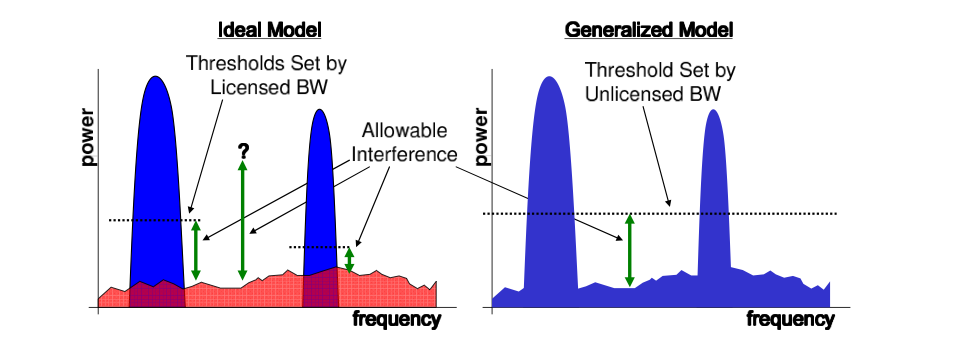
\includegraphics[width = \linewidth]{interferenceTemperatureModels.png}
\caption{Ideal and Generalized interpretations of the Interference Temperature Model. (Source: T. Charles Clancy, \emph{Formalizing the Interference Temperature Model}, Wiley Journal On Wireless Communications And Mobile Computing, 2006.)}
\end{figure}




\subsection*{Ideal model}

In the ideal model we try to guarantee that
\begin{equation}
    T_I(f_i,B_i) + \frac{M_iP}{kB_i} \leq T_L(f_i) \qquad \forall \quad 1 \leq i \leq n \label{idealModel}
\end{equation}
where, $T_L(f_i)$ is the interference temperature limit of the $i$'th receiver at center frequency $f_i$, $T_I(f_i,B_i)$ is  the interference temperature of the $i$'th receiver with center frequency $f_i$ and bandwidth $B_i$, $P$ is the power of the unlicensed transmitter, and $M_i$ is a constant between 0 and 1 representing the attenuation of the  transmitted power $P$ at the $i$'th receiver.

In words, equation \eqref{idealModel} means we try to keep the sum of the interference at the receiver (due to all other factors except the unlicensed transmitter) and the interference caused by the unlicensed transmitter's signal below the temperature limit $T_L$. Usually, a unified factor $M$ is used instead of $M_i$'s because we do not know the distance of every receiver. The factor $M$ is fixed by the regulators.

\subsubsection*{Challenges in implementing the ideal model}

\begin{itemize}
    \item It's hard to differentiate between licensed and unlicensed signals unless we already know the coexisting transmitters in the surrounding environment.
    \item It's difficult to measure the interference temperature $T_I$ in the presence of a licensed signal. We can determine the noise floor only when there is no signal power. For that we have to know when the signal power is going to be zero if it does. If the signal periodically goes to zero then we can measure the $T_I$ during the interval when it goes to zero. The other way is to take an average of the noise floor just outside the licensed signal band but we need to have information about the licensed signal's properties, like center frequency and bandwidth, to do that.
\end{itemize}


\subsection*{Generalized model}

The generalized model assumes that we have no a priori knowledge about the signal environment. Thus the constraint in this model has to be written in terms of the unlicensed transmitter's parameters.
\begin{equation}
    T_I(f_c,B) + \frac{MP}{kB} \leq T_L(f_c) \label{generalizedModel}
\end{equation}
where, $T_L(f_c)$ is the interference temperature limit of the unlicensed transmitter,
$T_I(f_c,B)$ is the interference temperature of the unlicensed transmitter, $P$ is the power of the unlicensed transmitter, and $M$ is a constant between 0 and 1 representing the factor by which the transmitted power gets attenuated.

If we constrain the transmitted power $P$ to be less than the one in the ideal model, from the equations \eqref{idealModel} and \eqref{generalizedModel} we get the following constraint,
\begin{equation}
    B(T_L - T_I(f_c,B)) \leq  B_i(T_L - T_I(f_i,B_i)) \qquad \forall \quad 1 \leq i \leq n \label{powerCompare}
\end{equation}
Suppose, every receiver receives a power $P_i$ and suppose the noise floor for all the receivers is the thermal noise temperature $T_N$, then we can rewrite the above equation \eqref{powerCompare} as,
\begin{align}
    BT_L - BT_I(f_c,B) & \leq  B_iT_L - B_iT_I(f_i,B_i) \nonumber\\  
    BT_L - B_iT_L & \leq BT_I(f_c,B) - B_iT_I(f_i,B_i) \nonumber\\  
    T_L(B- B_i) & \leq BT_I(f_c,B) - B_iT_I(f_i,B_i) \nonumber\\  
    T_L(B - B_i) + B_iT_I(f_i,B_i) & \leq  BT_I(f_c,B) \nonumber\\
    kBT_L(B - B_i) + kBB_iT_I(f_i,B_i) & \leq kB^2T_I(f_c,B) \nonumber\\  
    kBT_L(f_c)(B-B_i) + kBT_N\sum_{j=1}^{N}B_j & \leq \sum_{j=1}^{N}B_jP_j \qquad \forall \quad 1 \leq i\leq n
\end{align}

Though $T_I(f_c,B)$ can be measured easily, inclusion of all signals in its measurement gives rise to a more complex interference environment.


\section{Properties of Interference Temperature}

The problem with Interference Temperature model is that it is too simple. It tries to quantify interference assuming that interference behaves like noise. But interference doesn't actually behave like noise because we have defined interference to include all signals other than the one from the licensed transmitter. \emph{Interference Temperature} can't really model interference well enough.

The difference between the regulated temperature limit and the measured temperature is the amount of temperature that we are allowed to generate at the receiver. This temperature difference determines how much power our unlicensed transmitter can transmit to comply with the regulations.

The interference temperature $T_I$ can be written in terms of bandwidth $B$ as
\begin{align}
    T_I(f_c,B) & = \frac{1}{kB}P_I(f_c,B) \nonumber\\
    & = \frac{1}{kB}\left(\frac{1}{B}\int_{f_c-B/2}^{f_c+B/2}S(f)df\right) \nonumber\\
    & = \frac{1}{B^2k}\int_{f_c-B/2}^{f_c+B/2}S(f)df
\end{align}

The transmit power $P$ satisfying the general model can be found as
\begin{align}
    T_I(f_c,B) + \frac{MP}{kB} & \leq T_L(f_c) \nonumber \\
    \frac{MP}{kB} & \leq T_L(f_c) - T_I(f_c,B) \nonumber \\
    P & \leq \frac{kB}{M}T_L(f_c) - \frac{kB}{M}T_I(f_c,B) \nonumber \\
    P & \leq \frac{kB}{M}T_L(f_c) - \frac{1}{BM}\int_{f_c-B/2}^{f_c+B/2}S(f)df
    \label{maxtransmitpower}
\end{align}

We cannot find an explicit expression for $B$ satisfying the constraint. But if we consider the special case of $S(f) = c$ where $c$ is some constant, then the inequality \eqref{maxtransmitpower} can be rewritten as,
\begin{align}
    P & \leq \frac{kB}{M}T_L(f_c) - \frac{c}{M} \nonumber\\
    B & \geq \frac{PM + c}{kT_L(f_c)}
\end{align}
Thus now we have an expression for a minimum transmission bandwidth. Also the maximum transmit power turns out to be $kBT_L(f_c)$. As we increase $B$ the upper bound for transmit power increases. This implies that as we use more bandwidth we can produce more interference.


\section{Spectral analysis of radio signals}

The stimuli generated by radio emitters are nonstationary signals that depend on both time and space. But statistical analysis of nonstationary signals is complicated and cannot be implemented efficiently in practice. So, usually the incoming RF stimuli are sectioned into a continuous sequence of successive bursts, with each burst being short enough to justify pseudo-stationarity and yet long enough to produce an accurate spectral estimate\cite{haykin2009, haykin2005}.


A nonparametric spectral estimation method is required for this purpose and \emph{multitaper spectral estimation}\cite{haykin2009, thomson1982, percival1993} turns out to be the best choice. Multitaper spectral estimation has a nice property of allowing both reduced bias and reduced variance at the same time.

\subsection*{Multitaper spectral estimation}
This method uses \emph{multiple orthonormal tapers}\cite{haykin2009, thomson1982} to give different estimates of the spectrum. These estimates are then averaged to give the final estimate. This final estimate turns out to have both reduced bias and reduced variance\cite{haykin2009, thomson1982, percival1993}.


\begin{figure}
\centering
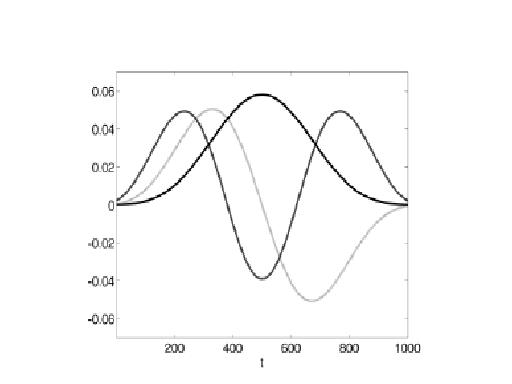
\includegraphics[width=0.65\linewidth]{DPSS_figure.jpg}
\caption{The three leading Slepian sequences for T=1000 and 2WT=6. Note that each higher order sequence has an extra zero crossing. [Source: http://en.wikipedia.org/wiki/Multitaper]}
\end{figure}




For a time series $\{x_t\}_{t=1}^N$, the multitaper spectral estimation procedure determines two things.
\begin{enumerate}
    \item $K$ orthonormal slepian tapers denoted by $\{w_t^{(k)}\}_{t=1}^{N}$
    \item The respective eigenspectra for each of the $K$ tapers
\begin{equation}
   Y_k(f) = \sum_{t=1}^N w_t^{(k)} x(t) e^{-j2\pi{}ft}, \qquad k = 0, 1, ...K-1
\end{equation}
\end{enumerate}

Most of the energy of the eigenspectra remain confined inside the \emph{resolution bandwidth}, denoted by $2W$ i.e. between $f-W$ and $f+W$. The \emph{time-bandwidth product}
\begin{equation}
    p = 2NW
\end{equation}
defines the \emph{degrees of freedom} available for controlling the variance of the spectral estimator.
A spectral estimate based on the first few eigenspectra with the least sidelobe leakage, is given by
\begin{equation}
    \hat{S}(f) = \frac{\sum_{k=0}^{K-1} \lambda_k(f) |Y_k(f)|^2}{\sum_{k=0}^{K-1} \lambda_k(f)}
\end{equation}
where $\lambda_k$ is the eigenvalue for the $k$th eigenspectrum. We can improve the spectral estimate by giving low weightage to the eigenspectra with more sidelobe leakage i.e. by choosing smaller $\lambda_k$'s for the higher $k$'s. This is called ``adaptive weighting''. The higher-order eigenspectra contain higher sidelobe leakage so we can weight them less.

\section{Estimation of interference temperature}
To get a reliable spectral estimate of the interference temperature, we do two things:
\begin{enumerate}
    \item Use the multitaper method to estimate the interference at the receiver and
    \item Use a lot of sensors to get a good approximation of the space dependent radio environment at the receiver. In case of mobile phones etc, we might have to stick to just one sensor.
\end{enumerate}


Suppose we have $M$ sensors then using $K$ different slepian tapers for each sensor we may form the $M$-by-$K$ matrix $\mathbf{A}(f)$, where the $\{w_m\}_{m=1}^M$ represent the weights attributed to the sensors.

\begin{equation}
    \mathbf{A}(f) = 
    \begin{bmatrix}
        w_1Y_1^{(1)}(f) & w_1Y_2^{(1)}(f) & \ldots & w_1Y_K^{(1)}(f) \\
        w_2Y_1^{(2)}(f) & w_2Y_2^{(2)}(f) & \ldots & w_2Y_K^{(2)}(f) \\
        \vdots & \vdots && \vdots \\
        w_MY_1^{(M)}(f) & w_MY_2^{(M)}(f) & \ldots & w_MY_K^{(M)}(f)
    \end{bmatrix}
\end{equation}

Each element in $\mathbf{A}(f)$ has contributions from both the additive internal noise and the incoming signal. We may get rid of the noise by using \emph{singular value decomposition}\cite{strang2009} to decompose $\mathbf{A}(f)$.

\begin{equation}
    \mathbf{A}(f) = \sum_{k=0}^{K-1} \sigma_k(f) \mathbf{u}_k(f) \mathbf{v}_k^{\dag}(f)
\end{equation}

We take the left singular vectors $\mathbf{u}_k(f)$ and the right singular vectors $\mathbf{v}_k(f)$ corresponding to the first few largest eigenvalues $|\sigma_k(f)|^2$. The first few largest eigenvalues $|\sigma_k(f)|^2$ provide a pretty good estimate of the interference temperature.



\bibliographystyle{plain}
\bibliography{interferenceTempEstimation}

\end{document}